\chapter{预备知识与相关工作}

本章中我们首先在 \S~\ref{sec:ch2-preliminaries} 介绍内外判定所需的广义环绕数及其离散表达，再说明其与复变函数、调和方程之间的联系；随后引入 Cauchy 变换、留数定理和双调和方程，奠定全文的数学基础；最后回到广义重心坐标、笼编辑与壳空间双射投影，为后续章节的方法推导建立统一的符号与理论基础。\S~\ref{sec:ch2-related-work} 结合文章的问题设置梳理相关工作的研究脉络；\S~\ref{sec:ch2-summary} 对本章内容与全文方法之间的对应关系作简要总结。
\section{预备知识}\label{sec:ch2-preliminaries}
\subsection{广义环绕数}
传统闭曲线的环绕数是平面内外判定中的经典概念。对二维有向闭合 Lipschitz 曲线 \(C\) 及查询点 \(p\in\mathbb{R}^2\setminus C\)，环绕数刻画了曲线围绕该点逆时针旋转的总次数，可写为
\begin{equation}
w_C(p)=\frac{1}{2\pi}\int_C d\theta.
\label{eq:ch2-gwn-def}
\end{equation}
这里 \(d\theta\) 表示曲线相对于查询点的极角微分。对简单闭曲线而言，环绕数在内部通常取 1，在外部取 0，因此可以直接用于内外判定；若存在自交或多重覆盖，则环绕数还能记录区域被包围的次数。

在此基础上，Jacobson 等人~\cite{Jacobson2013RobustIS} 将传统闭曲线的环绕数推广到了开放、非流形和存在重叠的曲线或曲面边界。推广后的广义环绕数沿用式 \eqref{eq:ch2-gwn-def} 的积分形式，但不再要求边界必须严格闭合。于是，当输入边界存在缝隙、重叠或非流形连接时，广义环绕数也不再只是一个严格的 0--1 指示函数，而是转化为一个更平滑的“内外置信度”量。

当 \(C\) 由分段线性线段组成时，式 \eqref{eq:ch2-gwn-def} 可以精确离散为各线段张角之和~\cite{Jacobson2013RobustIS}：
\begin{equation}
w_C(p)=\frac{1}{2\pi}\sum_{i=1}^{n}\theta_i(p),
\label{eq:ch2-gwn-polyline}
\end{equation}
其中 \(\theta_i(p)\) 为线段端点 \(c_i,c_{i+1}\) 相对于查询点 \(p\) 的有向夹角。若记
\[
\mathbf{a}=c_i-p,\qquad \mathbf{b}=c_{i+1}-p,
\]
则有
\begin{equation}
\tan \theta_i(p)=\frac{\det[\mathbf{a}\ \mathbf{b}]}{\mathbf{a}\cdot\mathbf{b}}.
\label{eq:ch2-gwn-angle}
\end{equation}
这说明二维广义环绕数可以直接由查询点到各边界线段的局部几何关系累加得到。

同样的思想也可以推广到三维。若闭曲面 \(S\) 由带定向三角形面片组成，则广义环绕数可以写成各面片张立体角的归一化和~\cite{Jacobson2013RobustIS}：
\begin{equation}
w_S(p)=\frac{1}{4\pi}\sum_{f=1}^{m}\Omega_f(p),
\label{eq:ch2-gwn-surface}
\end{equation}
其中 \(\Omega_f(p)\) 表示定向三角形面片 \(f\) 对查询点 \(p\) 的有向立体角。对三角形 \(f=(v_i,v_j,v_k)\)，记
\[
\mathbf{a}=v_i-p,\qquad \mathbf{b}=v_j-p,\qquad \mathbf{c}=v_k-p,
\]
并令 \(a=\|\mathbf{a}\|\)、\(b=\|\mathbf{b}\|\)、\(c=\|\mathbf{c}\|\)，则有
\begin{equation}
\tan \frac{\Omega_f(p)}{2}
=\frac{\det[\mathbf{a}\ \mathbf{b}\ \mathbf{c}]}
{abc+(\mathbf{a}\cdot\mathbf{b})c+(\mathbf{b}\cdot\mathbf{c})a+(\mathbf{c}\cdot\mathbf{a})b}.
\label{eq:ch2-gwn-solid-angle}
\end{equation}
因此，二维线段张角与三维三角形立体角构成了广义环绕数在分段线性边界上的两种基本离散单元，其几何关系见图~\ref{fig:ch2-gwn-projection}。

\begin{figure}[t]
  \centering
  \begin{overpic}[width=0.9\linewidth]{figures/chap2_gwn_projection.pdf}
    \put(18,0){\small \textbf{(a)}}
    \put(75,0){\small \textbf{(b)}}
    \put(14,15){\small \(p\)}
    \put(22,18){\small \(\theta\)}
    \put(36,10){\small \(c_i\)}
    \put(34,26){\small \(c_{i+1}\)}
    \put(53,10){\small \(v_i\)}
    \put(74,24){\small \(v_j\)}
    \put(62,32){\small \(v_k\)}
    \put(82,19){\small \(\Omega\)}
    \put(71,4){\small \(p\)}
  \end{overpic}
  \caption{广义环绕数在二维(a)与三维(b)中的几何示意。}
  \label{fig:ch2-gwn-projection}
\end{figure}

广义环绕数还具有两个对后续推导十分重要的性质。其一是可加性：若整体边界由若干有向曲线或曲面片组成，则总广义环绕数等于各部分贡献之和。其二是平移不变性：将查询点与边界同时按同一向量平移，不会改变广义环绕数的值。这意味着后续公式推导中可以不失一般性地将查询点平移至原点。

更重要的是，广义环绕数在边界之外是调和函数~\cite{Jacobson2013RobustIS}。对开放曲线或非水密曲面，它在边界两侧保持 \(\pm 1\) 的跳变，而在其余区域平滑变化。这一性质表明，广义环绕数与 Laplace 方程、复变函数和边界积分方法之间存在深刻联系，也是本论文后续将“内外判定”和“闭式积分求值”联系起来的关键出发点。

\subsection{柯西变换与留数定理}
在二维平面上，调和函数与复变函数之间存在天然对应：全纯函数的实部与虚部都是调和函数。基于这一点，Weber 等人~\cite{Weber2009} 从复分析出发，将边界上的控制信息通过 Cauchy 核传播到区域内部，从而构造了适用于平面变形的复重心坐标。对简单闭曲线 \(S=\partial\Omega\)、查询点 \(z\in\Omega\) 和边界点 \(w\in S\)，Cauchy 核为
\begin{equation}
C(w,z)=\frac{1}{2\pi i}\frac{1}{w-z},
\label{eq:ch2-cauchy-kernel}
\end{equation}
由此得到的 Cauchy 变换可写为
\begin{equation}
g_{S,f}(z)=\frac{1}{2\pi i}\int_{S}\frac{f(w)}{w-z}\,dw.
\label{eq:ch2-cauchy-transform}
\end{equation}
当边界函数 \(f\) 连续时，\(g_{S,f}\) 在 \(\Omega\) 内是全纯函数；若其导数不为零，则对应的平面映射是保角的。因此，Cauchy 变换既是边界数据到域内函数的传播机制，也为后续 Cauchy 坐标和 Green 坐标的解析表达提供了直接来源。

从经典复分析角度看，式 \eqref{eq:ch2-cauchy-transform} 建立在 Cauchy 积分公式之上。若 \(h\) 在 \(\Omega\subset\mathbb{C}\) 内全纯，且 \(\partial\Omega\) 为正向简单闭曲线，则对任意 \(z\in\Omega\) 有
\begin{equation}
h(z)=\frac{1}{2\pi i}\int_{\partial\Omega}\frac{h(\zeta)}{\zeta-z}\,d\zeta.
\label{eq:ch2-cauchy-integral}
\end{equation}
这说明全纯函数在区域内部的取值可以完全由边界积分确定。对几何处理而言，它提供了一条非常自然的思路：只在边界上给定控制量，再通过积分核将其传播到区域内部。

另一方面，留数定理则为这类边界积分的闭式求值提供了工具。若 \(a\) 是 \(F(z)\) 的 \(m\) 阶孤立奇点，则其留数为
\begin{equation}
\operatorname{Res}(F,a)=\frac{1}{(m-1)!}\lim_{z\to a}\frac{d^{m-1}}{dz^{m-1}}\!\left[(z-a)^mF(z)\right].
\label{eq:ch2-residue-def}
\end{equation}
若 \(\Gamma\) 为包围全部奇点的正向闭曲线，则
\begin{equation}
\oint_{\Gamma}F(z)\,dz=2\pi i\sum_k \operatorname{Res}(F,a_k).
\label{eq:ch2-residue-theorem}
\end{equation}
复平面中常用的积分路径构造见图~\ref{fig:ch2-residue-contour}。

\begin{figure}[t]
  \centering
  \begin{overpic}[width=0.62\linewidth]{figures/chap2_residue_path.pdf}
    \put(6,13){\small \(-a\)}
    \put(84,13){\small \(a\)}
    \put(92,13){\small 实轴}
    \put(50,60){\small 虚轴}
    \put(59,53){\small \(L_2\)}
    \put(52,23){\small \(L_1\)}
    \put(46,12){\small 奇点}
  \end{overpic}
  \caption{复平面中应用留数定理的典型积分路径示意。}
  \label{fig:ch2-residue-contour}
\end{figure}

对于本论文中的两类问题，这套复变工具链起到统一作用。在 Cauchy 坐标中，边界变形可通过式 \eqref{eq:ch2-cauchy-transform} 离散为各条边上的有理函数积分，并进一步转化为坐标权重及其导数的闭式表达~\cite{Weber2009,Lin2024PolynomialCC}。在曲线包含查询中，广义环绕数也可写成参数积分形式
\begin{equation}
w_{\gamma}(p)
=\frac{1}{2\pi}\int_0^1
\frac{x(t)y'(t)-y(t)x'(t)}{x^2(t)+y^2(t)}\,dt,
\label{eq:ch2-gwn-integral}
\end{equation}
再转化为复平面中的有理函数积分，并借助留数定理得到稳定的闭式求值公式。由此，广义环绕数与 Cauchy 变换虽然面向不同任务，但都可以归入“边界积分到域内求值”的统一框架之中。

\subsection{双调合方程}
广义环绕数在边界之外是调和函数，Cauchy 变换输出的全纯函数其实部和虚部也都是调和函数。因此，从广义环绕数到 Cauchy 坐标，后续多类方法的共同基础都是 Laplace 方程。然而，调和方程主要对应边界函数值的传播；当需要同时控制边界位置与边界导数时，就需要引入更高阶的双调和方程。

Weber 等人~\cite{Weber2012} 将双调和坐标表述为双调和 Dirichlet 问题。对平面区域 \(\Omega\)，设边界函数值与法向导数分别为 \(g_1,g_2\)，则对应的连续问题为
\begin{equation}
\Delta^2 f(x)=0,\quad x\in\Omega,
\label{eq:ch2-biharmonic-pde}
\end{equation}
并配以
\begin{equation}
f\big|_{\partial\Omega}=g_1,\qquad
\frac{\partial f}{\partial n}\Big|_{\partial\Omega}=g_2.
\label{eq:ch2-biharmonic-bc}
\end{equation}
在较弱条件下，该问题存在唯一解~\cite{Weber2012}。由于任意调和函数都是双调和函数，双调和方程可视为调和方程的自然推广；与此同时，它又允许同时插值边界值和边界导数，因此比调和方程具有更强的边界控制能力。

从变形角度看，双调和函数最直接的意义在于它把“仅控制边界位置”扩展为“同时控制边界位置与边界 Jacobian 的法向分量”。这使得双调和坐标不仅能传播位移信息，还能传播厚度、法向拉伸和边界附近的局部形变趋势。相应地，双调和坐标通常写为两组基函数的组合：一组负责边界值插值，另一组负责边界导数插值。后续第6章的高阶边界元构造，也正是建立在这一高阶边值问题之上。


进一步地，边界元方法（BEM）提供了求解双调和问题的一条自然路径：将域内 PDE 转化为边界积分方程，把未知量集中到边界自由度上，再通过边界离散进行求解~\cite{Weber2012,thiery2024biharmonic}。这不仅降低了未知量维度，也为后续高阶曲线边界上的双调和坐标构造提供了直接接口。

\subsection{广义重心坐标}
在上述数学基础之上，广义重心坐标提供了一种统一的“边界控制到域内传播”表达。重心坐标的基本思想是用控制点的仿射组合表示域内点。对线段端点 $v_1,v_2$，任意点 $x$ 可写为
\[
x=\lambda_1v_1+\lambda_2v_2,\qquad \lambda_1+\lambda_2=1.
\]
当 $x$ 位于线段内部时，$\lambda_1,\lambda_2\ge 0$，并可由距离比直接给出
\[
\lambda_1=\frac{\|v_2-x\|}{\|v_2-v_1\|},\qquad
\lambda_2=\frac{\|x-v_1\|}{\|v_2-v_1\|}.
\]
在线段情形基础上，二维三角形顶点 $v_1,v_2,v_3$ 的重心表示为
\[
x=\sum_{i=1}^3\lambda_i v_i,\qquad \sum_{i=1}^3\lambda_i=1,
\]
并可由面积比定义
\[
\lambda_i(x)=\frac{A(x,v_{i+1},v_{i+2})}{A(v_1,v_2,v_3)},
\]
其中 \(A(\cdot)\) 表示有向面积。该表示在单纯形上具有唯一性，并精确重现线性函数。
其几何意义见图~\ref{fig:ch2-simplex-barycentric}。

\begin{figure}[t]
  \centering
  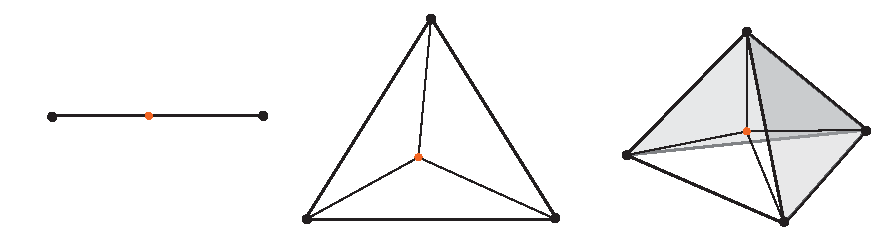
\includegraphics[width=0.90\linewidth]{figures/chap2_triangle_cor.pdf}
  \caption{三角形单纯形上的重心坐标示意。}
  \label{fig:ch2-simplex-barycentric}
\end{figure}

在实际几何编辑中，控制域通常是由闭合折线或曲面网格构成的包围几何，而非单纯形。因此需要引入广义重心坐标（Generalized Barycentric Coordinates, GBC）。设控制边界 \(C\) 的顶点为 \(\{c_i\}_{i=1}^{N}\)，其内部区域为 \(\Omega=\mathrm{Int}(C)\)。定义在 \(\Omega\) 上的一组标量函数 \(\{\lambda_i(x)\}\) 若满足
\begin{equation}
\sum_{i=1}^{N}\lambda_i(x)=1,
\label{eq:ch2-partition-of-unity}
\end{equation}
\begin{equation}
\sum_{i=1}^{N}\lambda_i(x)c_i=x,
\label{eq:ch2-linear-precision-position}
\end{equation}
则分别满足归一性与线性重现性。二者共同保证仿射不变性，也是各类笼坐标构造的共同基础。典型笼变形流程见图~\ref{fig:ch2-cage-gen}。

\begin{figure}[t]
  \centering
  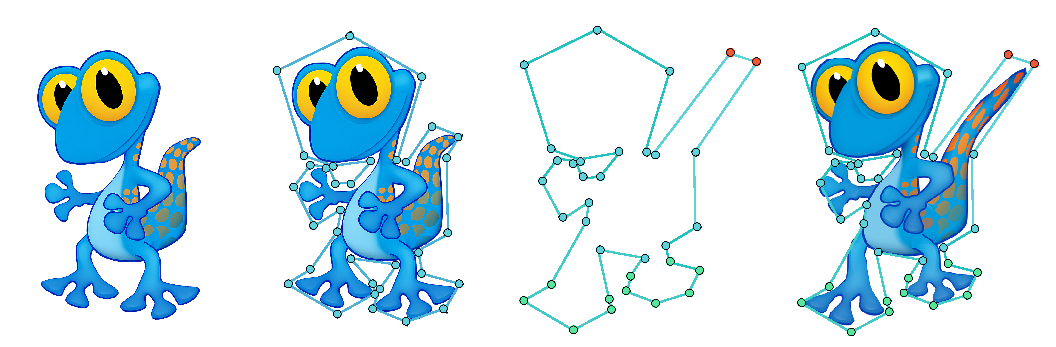
\includegraphics[width=0.96\linewidth]{figures/chap2_cage_gen.pdf}
  \caption{典型笼变形流程：构造笼、绑定坐标、编辑笼。}
  \label{fig:ch2-cage-gen}
\end{figure}

对模型顶点（或采样点）$v$，在绑定阶段预计算 \(\lambda_i(v)\)；在编辑阶段只需更新控制点位置 \(c_i'\)，即可得到
\begin{equation}
v'=\sum_{i=1}^{N}\lambda_i(v)c_i'.
\label{eq:ch2-cage-deform-basic}
\end{equation}
式 \eqref{eq:ch2-cage-deform-basic} 仅包含线性组合，因而适于高效并行计算。不同坐标方法的差异，主要体现在这些权重函数如何构造：均值坐标依赖几何角量，调和坐标来自 Laplace 方程，Cauchy/Green 坐标来自复变边界积分，而双调和坐标则进一步支持边界导数插值。也就是说，前面介绍的广义环绕数、复变积分与双调和方程，最终都可以理解为广义重心坐标家族中的不同数学来源。

\subsection{壳空间与双射投影}
\subsubsection{线性壳与高阶壳：等参映射与向量场约束}
在基于包围几何的另一条技术路线中，目标不是直接在边界上构造插值坐标，而是先建立一个可计算的三维包围空间，再在其中定义稳定的投影与属性传递。Jiang 等人~\cite{Jiang2020BijectivePI} 提出了“壳空间”与“双射投影”的统一框架。该框架的整体构造流程见图~\ref{fig:chap2-jiang-flow}。其将输入三角网格 \(T=\{V^T,F^T\}\) 转换为由广义棱柱组成的壳
\[
S=\{(B^S,M^S,T^S),F^S\},
\]
其中 \(B^S,M^S,T^S\) 分别表示壳的下、中、上表面，\(F^S\) 表示棱柱之间的连接关系。其核心在于在壳体内部定义体向量场 \(V\) 与投影算子 \(P\)，从而将壳内满足法向条件的曲面连续且双射地投影到中间曲面。

\begin{figure}[t]
  \centering
  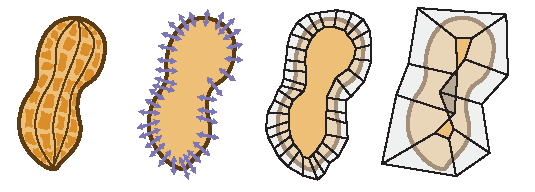
\includegraphics[width=0.78\linewidth]{figures/chap2_jiangshell.pdf}
  \caption{壳构造流程示意~\cite{Jiang2020BijectivePI}。}
  \label{fig:chap2-jiang-flow}
\end{figure}

对单个广义棱柱 \(\Delta\)，其几何由三组三角形顶点确定：上层顶点 \(\{t_1,t_2,t_3\}\)、下层顶点 \(\{b_1,b_2,b_3\}\)，以及由参数 \(\alpha_i\in[0,1]\) 插值得到的中层顶点
\[
m_i=\alpha_i t_i+(1-\alpha_i)b_i,\quad i=1,2,3.
\]
为得到可计算的投影映射，\(\Delta\) 被分解为 6 个四面体，并在每个四面体内部定义常向量场。若点 \(p\) 位于某个四面体 \(T_j^\Delta\) 中，则其向量场取值可写为
\[
V(p)=t_i-b_i,
\]
其中 \(i\) 对应该四面体所属的柱边索引。投影算子 \(P\) 定义为沿 \(V\) 的积分线追踪点 \(p\)，并取其与棱柱中间面的交点。广义棱柱的分解与壳内投影向量场示意见图~\ref{fig:chap2-jiang-prism}。

\begin{figure}[t]
  \centering
  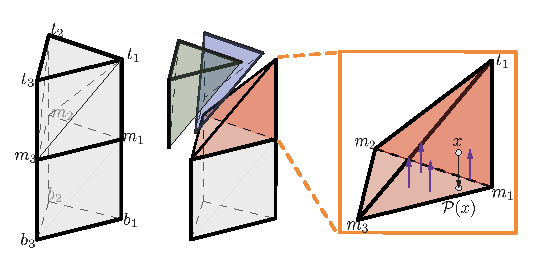
\includegraphics[width=0.70\linewidth]{figures/chap2_jiangprism.pdf}
  \caption{广义棱柱分解与壳内投影向量场示意~\cite{Jiang2020BijectivePI}。}
  \label{fig:chap2-jiang-prism}
\end{figure}

在上述构造基础上，若网格 \(\hat T\) 与棱柱 \(\Delta\) 的交集满足连通边界条件，且对任意交点 \(p\) 都有
\[
\langle n(p),V(p)\rangle>0,
\]
则称 \(\hat T\) 是 \(\Delta\) 的一个截面；若对壳内每个棱柱都成立，则称 \(\hat T\) 是壳 \(S\) 的截面。法向一致性与正体积条件共同保证壳空间的有效性，而由投影算子诱导的截面间映射则保证双射。这一框架与前述基于边界的坐标方法互补：前者提供可计算的包围空间，后者提供边界到域内的函数传播，二者共同构成本文后续方法的基础。
\section{相关工作}\label{sec:ch2-related-work}
\subsection{包含查询}
包含查询是几何处理中的基础问题。对多边形区域，基于射线交点奇偶性或环绕数累积的判定策略已有长久历史，相关实用算法可追溯到19世纪60年代~\cite{Shimrat1962Algorithm1P,Haines1994Point,Carvalho1995}。当边界由 B\'{e}zier 曲线、修剪曲面或更一般的 NURBS 给出时，问题会迅速变得复杂，因为查询过程不再只是线段相交计数，而需要同时处理参数表示、裁剪和数值稳健性~\cite{Nishita1990RayTT,1997The,Marussig2017ARO}。在 CAD/CAE 场景中，若简单用分段线性边界近似曲边，还可能把几何误差进一步传递到后续数值计算中~\cite{Sevilla2008NURBSenhancedFE}。

从拓扑角度看，闭曲线环绕数的概念可追溯到经典数学文献~\cite{meister1771generalia}。Jacobson 等人~\cite{Jacobson2013RobustIS} 提出的广义环绕数将传统整数值环绕数扩展到可能非水密、非流形或存在重叠的曲线与曲面边界，使其不仅能对规则闭区域完成内外判定，也能在不完美输入上给出平滑的置信度场。近年来，围绕环绕数字段的可微化与场表示也出现了新的工作，例如通过高斯核卷积构造可微环绕数及其导数~\cite{Sun2024GauWNGW}。射线法与广义环绕数法的直观判定方式见图~\ref{fig:ch2-containment-query}。

\begin{figure}[t]
	\centering
	\begin{overpic}[width=0.96\linewidth,percent]{figures/chap2_RayCasting.pdf}
	\end{overpic}
	\caption{内外判断用于确定查询点相对于包围边界位于内部还是外部。左图为射线法，通过统计射线与边界交点的奇偶性完成判定；右图为广义环绕数法，通过累积边界绕查询点的旋转量完成判定。图中标出了内部区域与外部区域。}
	\label{fig:ch2-containment-query}
\end{figure}

对于需要显式处理曲边内域的任务，如角色皮肤弹性仿真、扩散曲线表示与自由手绘编辑，稳定的包含查询不仅是预处理步骤，也是后续场计算的一部分~\cite{McAdams2011EfficientEF,Orzan2013DiffusionCA,Scrivener2024WindingNF}。

在几何对象类型上，广义环绕数已经从三角网格扩展到点云、离散曲面以及参数曲线和曲面。Barill 等人~\cite{Barill2018} 将其用于点云的内外判定，Feng 等人~\cite{Feng2023WindingNO} 讨论了离散曲面上的环绕数字段，而 Spainhour 等人~\cite{Spainhour2024RobustCQ} 与 Martens 等人~\cite{Martens2024OneShotMF} 则将这一思路推广到有理参数曲线和曲面。对曲边边界而言，这一路线尤其重要，因为传统射线法和分段线性近似在精度、鲁棒性与效率之间往往难以兼顾。现有面向有理曲线的广义环绕数方法能够取得较高精度，但由于缺乏闭式求值形式，其计算代价会随着曲线形状和查询点位置显著变化~\cite{Spainhour2024RobustCQ}。

广义环绕数的应用也已超出单纯的内外判定。它被用于二维图像中的显著轮廓检测~\cite{Ming2015WindingNC} 与颜色传播~\cite{Scrivener2024WindingNF}，也被用于从线性网格或点云生成体网格~\cite{Jacobson2013RobustIS,Barill2018}。由于环绕数字段在边界之外平滑变化，还能为精确网格布尔运算提供良好的局部性和稳健性~\cite{Trettner2022EMBER}。最近，这类方法还被用于浸入式几何分析，以支持围绕非结构化点云几何对象的流体计算~\cite{Balu2023}。总体来看，包含查询相关研究正从“判定一个点是否在内部”逐步发展为“在复杂边界上构造稳定、可微且可用于后续计算的内外场”。

\subsection{包围几何生成与应用}
包围几何（壳/笼）是数字几何处理中一类重要的中间表示。其一项核心用途是在重网格化中作为“误差控制层”，约束新网格始终位于允许的几何偏差范围内~\cite{hu2019TriWild,cheng2019practical,hu2020fast}；另一项重要用途是在边界附近构造一个可计算空间，从而支持属性传递、贴图、布尔运算和后续数值处理。围绕这一思路，包围几何的应用已覆盖渲染中的壳映射与 2.5D 纹理表示~\cite{chen2004shell,hormann2007mesh,jin2019shell,lengyel2001real,peng2004interactive,porumbescu2005shell,wang2003view,wang2004generalized}、流体计算中的边界层网格生成~\cite{aubry2017boundary,garimella2000boundary}，以及碰撞检测与动画控制中的代理结构~\cite{calderon2017bounding,thiery2012cager}。

\citet{Jiang2020BijectivePI} 将这一思路系统化，提出带有双射投影的线性壳结构。与仅用于限制几何误差的传统包络 或 边界层 不同，该框架不仅构造了围绕输入曲面的包围空间，还在壳内显式定义了连续投影，使输入曲面与壳内截面之间能够稳定地传递属性。因此，线性壳不仅可服务于重网格化，还可直接用于位移贴图构建、布尔运算和四面体网格生成等任务。围绕同一目标，\citet{liu2024curveshell} 将线性壳推广到高阶壳：每个单元由上、中、下三张 B\'{e}zier 三角面与侧双线性曲面围成的广义棱柱构成。从更一般的高阶网格视角看，B\'{e}zier 三角形与 B\'{e}zier 四面体等高阶单元已被广泛用于边界拟合和高阶数值分析~\cite{farin1986triangular,mandad2020bezier,Dey99curvilinearmesh,Ferguson2022HighOrderIP,Ruiz-Giron2021Measure}；相应生成流程通常遵循“先线性离散、再曲化或优化”的路线~\cite{LIU2021103080,Jiang2021Bijectiveandcoarse,Xu2014,Jiang2021BijectiveAC}。

从应用角度看，可以在壳内执行重网格化，并通过双射投影实现输入网格与新网格之间的属性往返传递；可以在高质量重网格上完成距离场等数值计算，再稳定地传回原始网格；也可以在壳内完成并集等操作、构建位移贴图，或在简化网格上计算向量场后再映射回高分辨率模型。对应应用示例分别见图~\ref{fig:ch2-shell-proxy} 和图~\ref{fig:ch2-shell-displace}。与显式壳结构并行，属性传递还常借助连续法向投影或共享基域映射建立对应。前者包括位移贴图与可逆投影等方法~\cite{lee2000displaced,Kobbelt1998InteractiveMM,ezuz2019reversible,panozzo2013weighted}；后者则通过圆盘、平面域、粗多面体、轨形、Poincar\'{e} 圆盘、谱基和抽象基域上的参数化来传播属性~\cite{tutte1963draw,floater1997parametrization,surazhsky2001morphing,jiang2017simplicial,kraevoy2004cross,praun2001consistent,aigerman2017spherical,jin2008discrete,kharevych2006discrete,shoham2019hierarchical,pietroni2009almost,hormann2017generalized}。这些方法在跨表面映射和形状对应中十分重要~\cite{JiaoInternationalJO,kraevoy2004cross,Ovsjanikov_Ben-Chen_Solomon_Butscher_Guibas_2012}，但当目标是围绕输入边界构造一个可计算、可保证双射的局部空间时，仍需要壳结构这类更强的几何约束。

\begin{figure}[t]
  \centering
  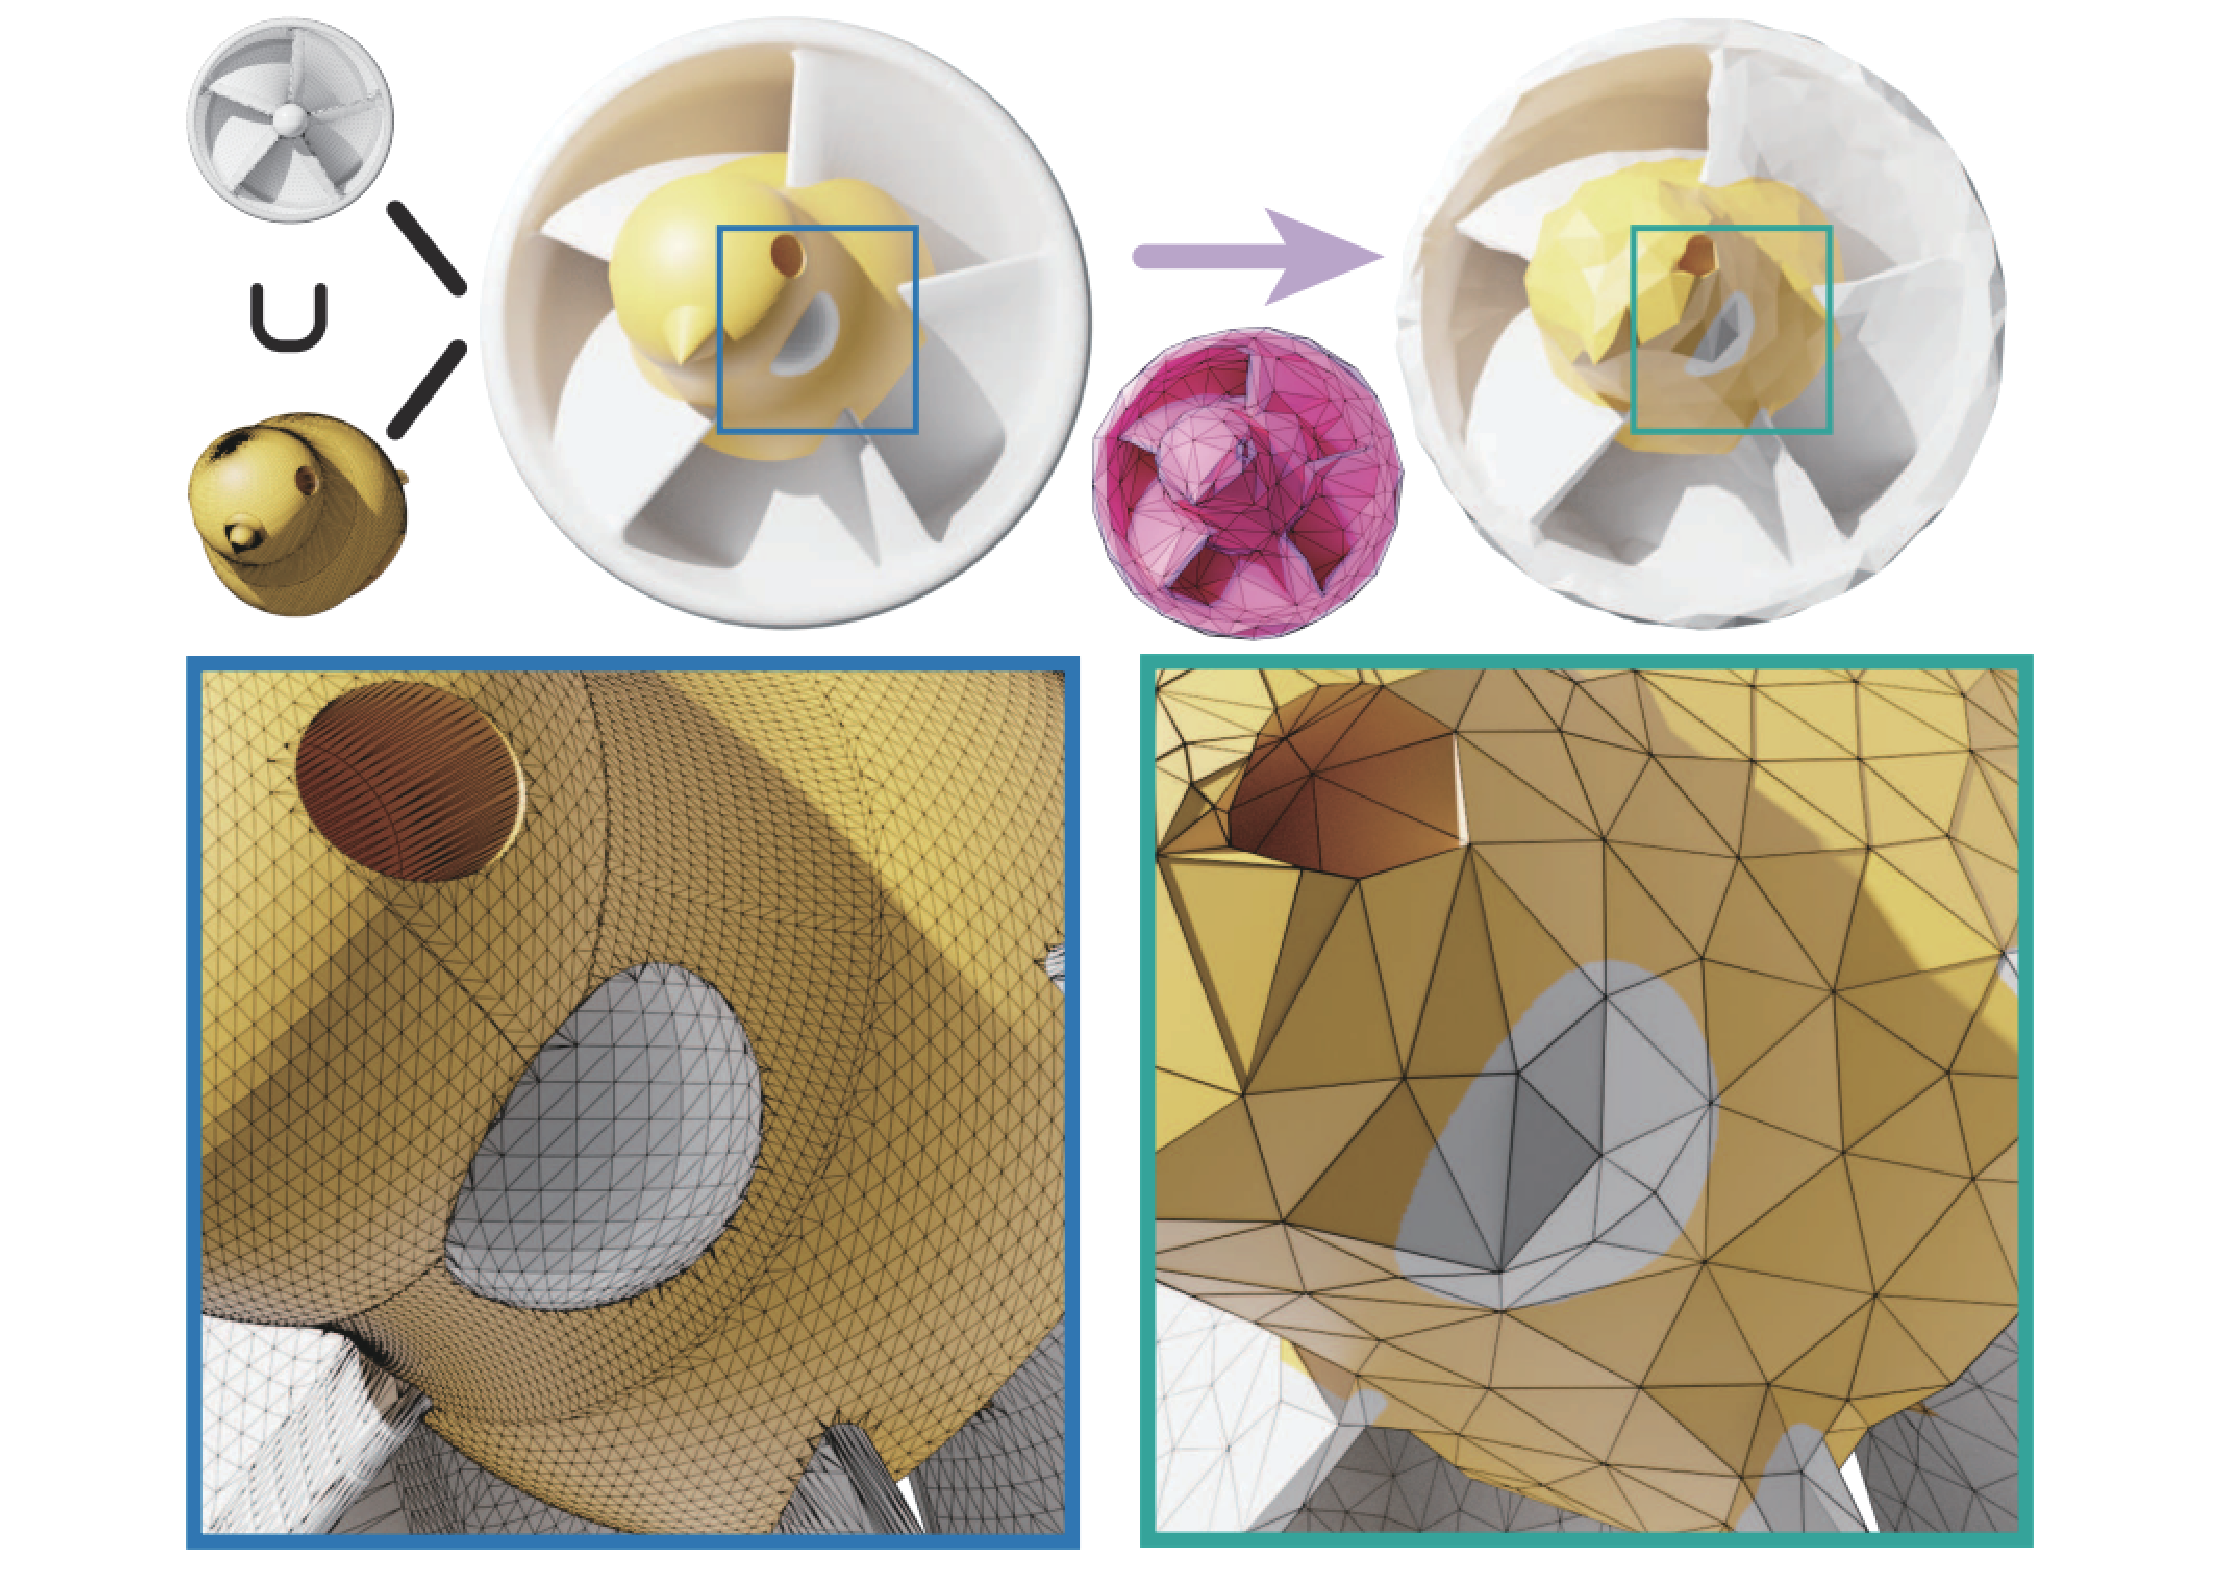
\includegraphics[width=0.58\linewidth]{figures/chap2_proxy.pdf}
  \caption{壳在“重网格化计算-回传”流程中的应用实例\cite{Jiang2020BijectivePI} 。}
  \label{fig:ch2-shell-proxy}
\end{figure}

\begin{figure}[t]
  \centering
  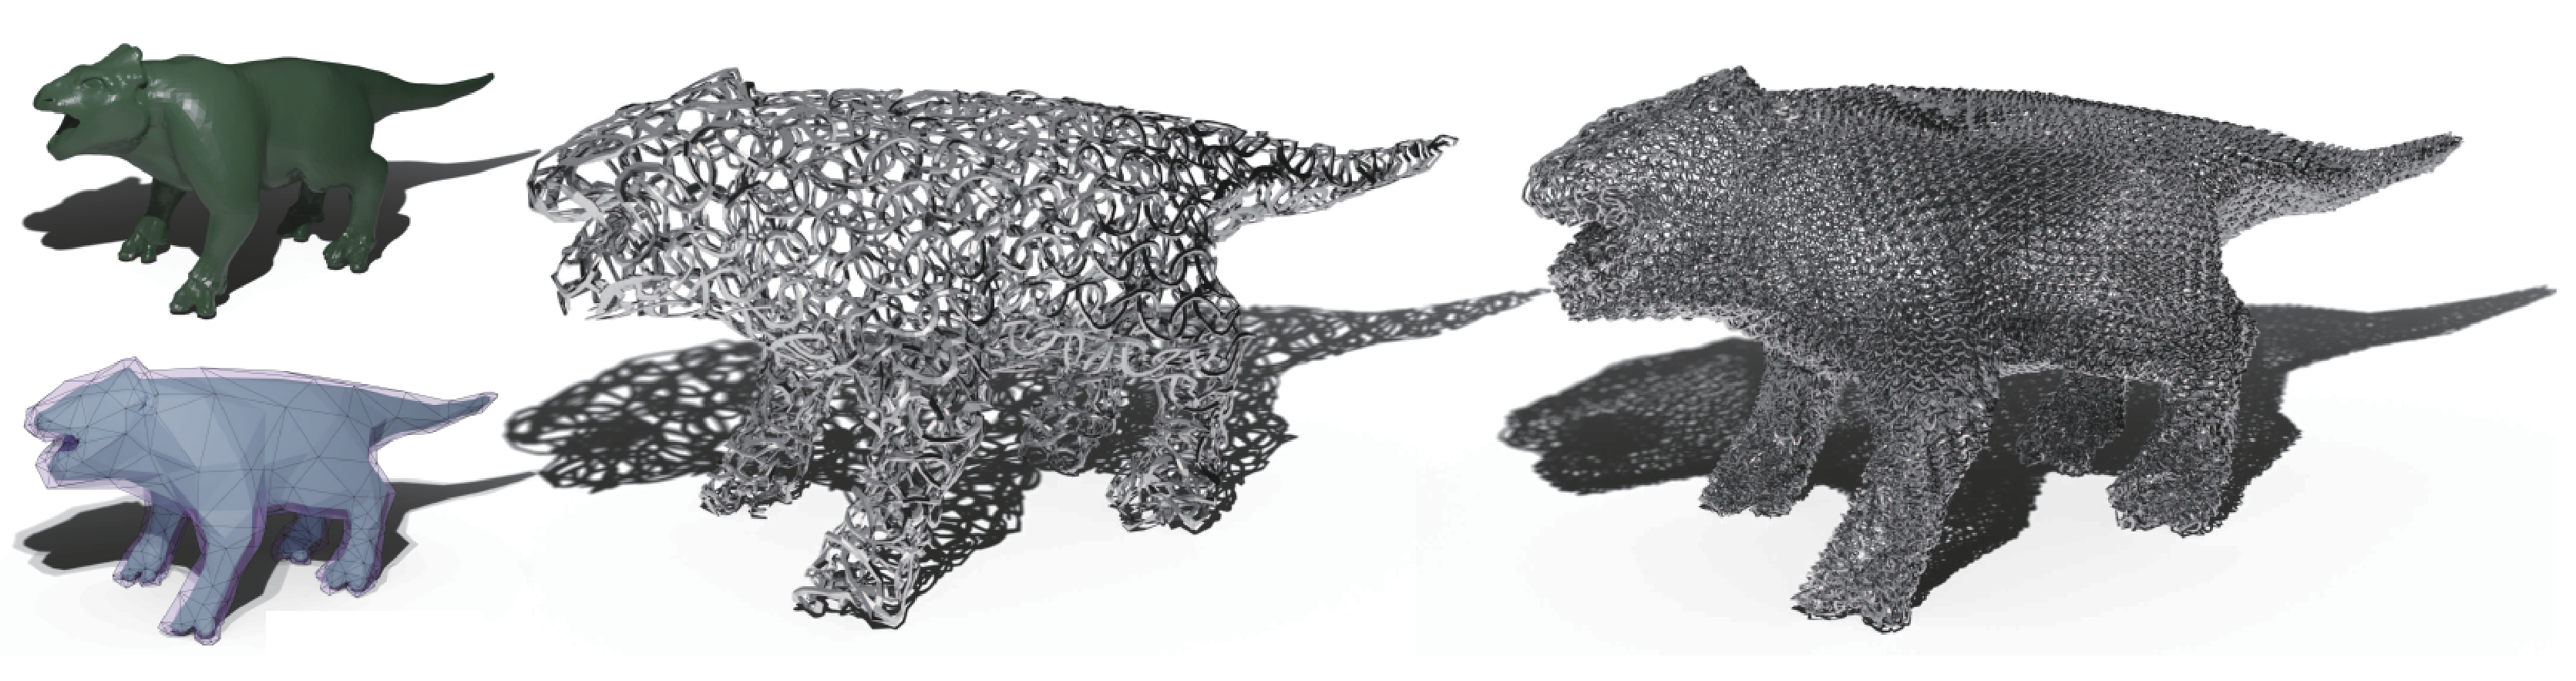
\includegraphics[width=0.98\linewidth]{figures/chap2_displace.pdf}
  \caption{壳投影用于位移贴图构建的应用示例\cite{Jiang2020BijectivePI}。}
  \label{fig:ch2-shell-displace}
\end{figure}

另一条相关路线是在重网格化过程中显式追踪前后对应，通过 重叠三角化、连续参数化和 内蕴三角化 等机制维持映射关系~\cite{Sharp2019NavigatingIT,Schmidt2020IntersurfaceMV,Gillespie2021IntegerCF,cohen1997simplifying,Lee1998MAPSMA,Liu2020NeuralS,Liu2023SurfaceSU,Sharp2021GeometryPW}。与这类“沿操作追踪对应”的思路相比，壳/笼更强调先构造稳定的空间代理，再在其中定义统一的投影和传递算子。

\begin{figure}[t]
  \centering
  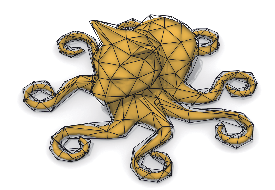
\includegraphics[width=0.62\linewidth]{figures/chap2_robustcage.pdf}
  \caption{鲁棒粗笼构造工作中的包围几何结果示例\cite{Guo2024RobustCage} 。}
  \label{fig:ch2-robustcage}
\end{figure}

围绕“自动生成笼结构”这一问题，已有方法多面向直边笼，如第一章所示。另一方面，\citet{Edelstein2025CageNet} 将笼视为学习与推理之间的桥接域，针对原始网格自动构造外包笼，并通过从笼到输入网格的映射算子提升分割与蒙皮任务中的泛化能力。典型包围结果见图~\ref{fig:ch2-robustcage}。总体来看，包围几何生成与应用相关研究可概括为两条互补路径：一条路径强调如何围绕输入构造有效、无自交、可优化的壳/笼；另一条路径强调如何利用这些包围结构服务于属性传递、数值求解、渲染、布尔和学习等下游任务。本文同时关注包围几何的生成质量与其作为计算域的可用性。

\subsection{广义重心坐标}
广义重心坐标为“由边界控制点向域内传播信息”提供了统一框架。设闭合控制多边形（或多面体）为 \(C\)，其控制点为 \(\{c_i\}_{i=1}^{m}\)，内部区域为 \(\Omega\)。定义在 \(\Omega\) 内部的标量函数 \(\{\lambda_i(x)\}\) 通常满足前文式~\eqref{eq:ch2-partition-of-unity} 和式~\eqref{eq:ch2-linear-precision-position} 所示的归一性与线性重现性。在笼变形中，先在绑定阶段计算模型点 \(v\) 的权重 \(\lambda_i(v)\)，再在编辑阶段更新控制点位置 \(c_i'\)，即可按式~\eqref{eq:ch2-cage-deform-basic} 得到变形后的位置 \(v'\)。这一表达构成了“坐标绑定-控制点编辑-形状更新”的统一框架。围绕这一框架，研究者发展出了不同性质的坐标构造，它们主要在闭式性、非负性、平滑性、局部性以及边界控制能力之间进行权衡。

在二维图像与矢量图形编辑中，笼变形并不是唯一方案。自由形变、移动最小二乘和基于基本解的刷式编辑分别从控制网格、局部拟合和弹性核函数角度提供了另一组代表性框架~\cite{Sederberg1986,Schaefer2006,DeGoes2017}。不过，当需求是将边界控制稳定地传播到整个区域内部时，广义重心坐标仍是最系统、最可组合的一类方法。

\paragraph{均值坐标（Mean Value Coordinates）}
对二维多边形笼，均值坐标给出了闭式权重表达，可高效实现插值变形~\cite{Floater2003,Hormann2006,Ju2005}。设 \(x\) 为内部查询点，\(\alpha_i\) 表示 \(x\) 处由相邻控制点张成的角，则常用写法为
\begin{equation}
w_i(x)=\frac{\tan(\alpha_{i-1}/2)+\tan(\alpha_i/2)}{\|c_i-x\|},\qquad
\lambda_i(x)=\frac{w_i(x)}{\sum_{j=1}^{m} w_j(x)}.
\end{equation}
均值坐标具有闭式形式，实现简单，并在凸笼上表现稳定；其闭式性也使其适合多分辨率与实时编辑框架~\cite{Huang2006,Farbman2009}。相关坐标函数与形变响应示意见图~\ref{fig:ch2-hc-page}。但在强凹区域可能出现负权重，进而产生不符合直觉的局部拉扯现象。

\paragraph{调和坐标（Harmonic Coordinates）}
为改善均值坐标在凹形区域中的表现，调和坐标将权重定义为 Laplace 方程的解~\cite{Joshi2007,Lipman2007}：
\begin{equation}
\Delta \lambda_i(x)=0,\quad x\in\Omega,\qquad
\lambda_i(x)\big|_{\partial\Omega}=g_i(x),
\end{equation}
其中 \(g_i\) 是边界上的插值条件。由于满足最大值原理，调和坐标在内部具有更好的平滑性与稳定性，并能显著减弱远距离的不合理耦合。

\begin{figure}[t]
  \centering
  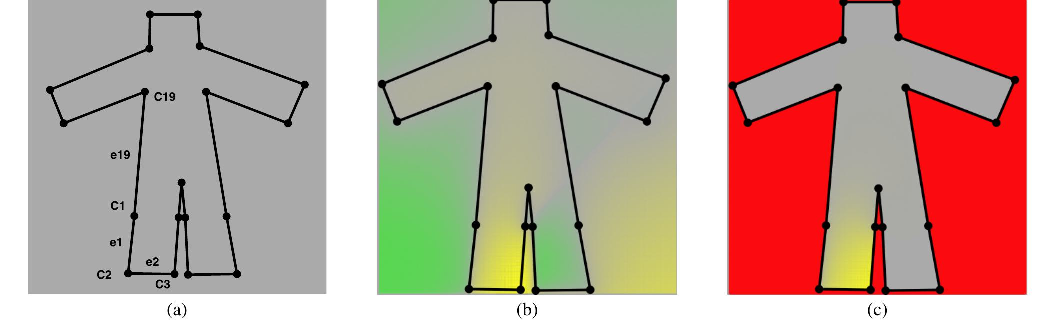
\includegraphics[width=0.95\linewidth]{figures/chap2_harmonic_coordinates_weights.pdf}
  \caption{调和坐标示意图：凹形域中的坐标函数与形变响应~\cite{Joshi2007,Lipman2007}。}
  \label{fig:ch2-hc-page}
\end{figure}

在插值型坐标内部，Poisson 坐标、最大熵坐标、最大似然坐标、局部重心坐标和变分重心坐标分别从逼近精度、非负性、统计解释、局部性和能量最优等角度推进了这一方向~\cite{li2012poisson,Hormann2008Maximum,Chang2023Maximum,Zhang2014Local,Dodik2023Variational}。这些方法通常不具备与均值坐标同样简洁的闭式表达，但能在特定任务中提供更强的边界控制或更局部的响应。

\paragraph{Green 坐标与 Cauchy 坐标}
在这一脉络下，Green 坐标与 Cauchy 坐标可视为“边界积分型坐标”的代表~\cite{Lipman2008,Weber2009}。这类方法不仅使用边界位置信息，还引入边界法向（或导数）信息，以增强局部保形能力。其典型表达可写为
\begin{equation}
f(x)=\sum_i \phi_i(x)c_i+\sum_j \psi_j(x)\mathbf{n}_j,
\end{equation}
其中 \(\phi_i,\psi_j\) 分别对应位置项与法向项的权重，\(\mathbf{n}_j\) 为边界法向（或边界导数方向）量。对应到复平面，Cauchy 形式常写为
\begin{equation}
f(z)=\frac{1}{2\pi i}\int_{\partial\Omega}\frac{f(\zeta)}{\zeta-z}\,d\zeta,
\end{equation}
并据此导出具有保角特性的二维权重表达。

除 Green/Cauchy 坐标外，Somigliana 坐标~\cite{chen2023somigliana}将线弹性边界积分引入笼变形，以获得体积控制能力。在矢量图形场景中，Poisson矢量图~\cite{Hou2017}也采用闭式边界传播来联合处理颜色与梯度约束，说明边界积分思想并不只服务于几何位置插值。

\paragraph{双调和坐标（Biharmonic Coordinates）}
双调和坐标将“边界值插值”推广为“边界值+边界法向导数”的联合插值~\cite{Weber2012}。常见形式为
\begin{equation}
f(x)=\sum_{i=1}^{m}\alpha_i(x)f_i+\beta_i(x)d_i,
\end{equation}
其中 \(f_i\) 是边界控制值，\(d_i\) 是边界法向导数数据。其 Hermite 型边界条件可写为
\begin{equation}
\alpha_i(v_j)=\delta_{ij},\quad \beta_i(v_j)=0,\quad
\frac{\partial \alpha_i}{\partial n}\Big|_{e_j}=0,\quad
\frac{\partial \beta_i}{\partial n}\Big|_{e_j}=\delta_{ij},
\end{equation}
并在域内满足双调和方程
\begin{equation}
\Delta^2\alpha_i(x)=0,\qquad \Delta^2\beta_i(x)=0,\qquad x\in\Omega.
\end{equation}
与调和坐标相比，双调和坐标允许更丰富的边界控制自由度，因此在形状编辑中更容易兼顾平滑性与局部细节响应。与其他变形方法的典型对比见图~\ref{fig:ch2-biharmonic-page-related}。类似思路也被用于 扩散曲线 的双调和边界元表达~\cite{Ilbery2013}。

\begin{figure}[t]
  \centering
  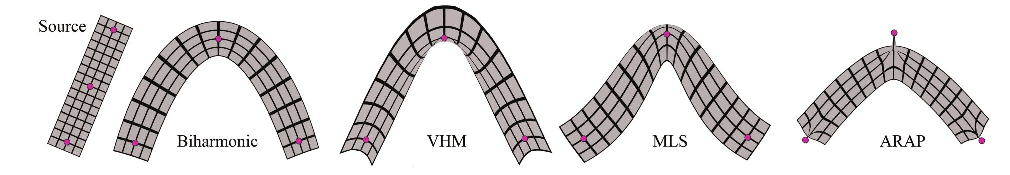
\includegraphics[width=0.95\linewidth]{figures/chap2_biharmonic_coordinates_teaser.pdf}
  \caption{双调和坐标与其他变形方法对比示意~\cite{Weber2012}。}
  \label{fig:ch2-biharmonic-page-related}
\end{figure}

随着高阶边界表示的普及，B\'{e}zier 三角形、B\'{e}zier 四面体及其有理变体被广泛用于高精度边界拟合~\cite{farin1986triangular,mandad2020bezier,Mandad2021Guaranteed,Yang2022PreciseHM,Khanteimouri2022RationalBG,Jiang2021BijectiveAC}；但自动笼生成方法仍多面向直边结构~\cite{Sacht2015,Guo2024RobustCage}。相应地，坐标系统也开始从多边形或多面体推广到高阶笼：三次均值坐标与 Coons 型推广增强了插值型曲边编辑能力~\cite{Li2013,Qin2024Coons}，而多项式 Green/Cauchy 坐标及其直接面向高阶输入笼的推广，则在保持闭式表达的同时延续了保形或近保形性质~\cite{MichelThiery2023,Lin2024PolynomialCC,liu2024polygc}。

从求解角度看，边界元方法在图形学中已被用于实时可变形体、海浪、表面液体、体内方向场与平面调和映射等问题~\cite{James1999ArtDefoAR,Schreck2019,Da2016SurfaceonlyL,Solomon2017BoundaryEO,Levi2016OnTC}，也支撑了扩散曲线与大规模边界求解器的发展~\cite{Bang2023,Chen2024LightningfastMO}。进一步地，近期工作已将双调和坐标推广到三维网格笼与更一般的离散边界，并在求解层面采用边界元框架统一处理插值条件与导数条件~\cite{thiery2024biharmonic}。相较于线性边界单元，这一路线在复杂边界上具有更好的几何拟合能力与变形稳定性，也为高阶笼上的构造提供了直接的数值支撑。由此来看，广义重心坐标相关研究已经形成从均值坐标、调和坐标，到 Green/Cauchy 坐标，再到双调和坐标、高阶笼扩展与边界元求解的一条连续发展脉络。

\section{本章小结}\label{sec:ch2-summary}
本章围绕后续四章的方法需求，梳理了统一的理论基础与研究背景。预备知识部分按照“广义环绕数-复变工具-双调和方程-笼坐标-壳空间”的顺序，介绍了内外判定、边界积分、边值问题与双射投影的共同数学基础，为第3章的内外判断、第4章的壳内投影、第5章的柯西坐标闭式推导和第6章的高阶 BEM 构造建立了统一接口。相关工作部分则重组为“包含查询-包围几何生成与应用-广义重心坐标”三条脉络，分别对应本文在内外判定、包围空间构造与边界插值上的研究背景。
